%%%%%%%%%%%%%%%%%%%%%%%%%%%%%%%%%%%%%%%%%
% Short Three-Column Newsletter
% LaTeX Template
% Version 1.0 (11/9/13)
%
% Original author:
% Frits Wenneker (http://www.howtotex.com) 
% With extensive modifications by:
% Vel (vel@latextemplates.com)
% 
% This template has been downloaded from:
% http://www.LaTeXTemplates.com
%
% License:
% CC BY-NC-SA 3.0 (http://creativecommons.org/licenses/by-nc-sa/3.0/)
%
%%%%%%%%%%%%%%%%%%%%%%%%%%%%%%%%%%%%%%%%%

%----------------------------------------------------------------------------------------
%	PACKAGES AND DOCUMENT CONFIGURATIONS
%----------------------------------------------------------------------------------------

\documentclass[10pt,a4paper,ngerman,twoside]{article} % Paper type (a4paper, usletter or legal) and font size (10, 11 or 12)

%\setlength\topmargin{-80mm} % Top margin
\setlength\topmargin{-48pt} % Top margin
\setlength\headheight{0pt} % Header height
\setlength\textwidth{7.0in} % Text width
\setlength\textheight{9.5in} % Text height
\setlength\oddsidemargin{-30pt} % Left margin
\setlength\evensidemargin{-30pt} % Left margin (even pages) - only relevant with 'twoside' article option
%\setlength\inner{4cm}
%\setlenfth\outer{2cm}
%\usepackage{geometry}
%\geometry{bindingoffset=20mm}
%\setlength\bindingoffset{2cm}

\usepackage{charter} % Charter font for main content

\frenchspacing % Reduces space after periods to make text more compact for a three-column layout
\usepackage{babel}
\usepackage[utf8]{inputenc}
\usepackage{graphicx} % Required for including images
\usepackage{amssymb} % Math packages
\usepackage{amsmath} 
\usepackage{multicol} % Required for the three-column layout of the document
\usepackage{url} % Clickable links
\usepackage{enumitem} % Reduces the amount of space within and between lists with [noitemsep,nolistsep]
\usepackage{marvosym} % Required for the use of symbols
\usepackage{wrapfig} % Allows wrapping text around figures
%\usepackage[T1]{fontenc} % Use 8-bit encoding that has 256 glyphs
\usepackage{datetime} % Required for defining a custom date style
\newdateformat{mydate}{\monthname[\THEMONTH] \THEYEAR} % Set a custom date format
\usepackage[pdfpagemode=FullScreen, colorlinks=false]{hyperref} % Link colors and PDF behavior in Acrobat
\usepackage{fancyhdr} % Required to define custom headers/footers
\usepackage{hyperref} % funktioniert nicht ?
\pagestyle{fancy} % Enables the custom headers/footers for all pages following this

%-----------------------------------------------------------
% Header and footer
\lfoot{\footnotesize % Left footer containing newsletter contact information
%\begin{wrapfigure}{l}{2.0cm}
%
\includegraphics[width=2cm]{ccbysa88x31.png} 
%\end{wrapfigure}
R.I.S. Journal Ausgabe 001, Jänner 2014: \textbf{R}emix, \textbf{I}mprove, \textbf{S}hare. Das freie, creativ-commons lizensierte Journal.  \\
\Mundus\ Download und andere Formate: \href{http://spielend-programmieren.at/de:ris:start}{\texttt{spielend-programmieren.at/de:ris:start}} \quad
%\Telefon\ (000) 111-1111 \quad
\Letter\ \href{mailto:horst.jens@spielend-programmieren.at}{horst.jens@spielend-programmieren.at}
}

\cfoot{} % Empty center footer

\rfoot{\footnotesize ~\\ Seite \thepage} % Right footer - page counter

\renewcommand{\headrulewidth}{0.0pt} % No horizontal rule for the header
\renewcommand{\footrulewidth}{0.4pt} % Horizontal rule separating the footer from the document
%-----------------------------------------------------------

%-----------------------------------------------------------
% Define separators
\newcommand{\HorRule}[1]{\noindent\rule{\linewidth}{#1}} % Creates a horizontal rule
\newcommand{\SepRule}{\noindent	% Creates a shorter separator rule
\begin{center}
\rule{250pt}{1pt} % Page width and rule width
\end{center}
}
\newcommand{\Trenner}{\noindent
\begin{center}
\rule{100pt}{1pt}
\end{center}
}
%-----------------------------------------------------------

%-----------------------------------------------------------
% Define title and article styles
\newcommand{\NewsletterName}[1]{ % Newsletter title
\begin{center}
\Huge \usefont{T1}{fvs}{b}{n} % Use the Bera Sans Bold font
#1
\end{center}	
\par \normalsize \normalfont}

\newcommand{\JournalIssue}[1]{ % Date and issue number at the top of the newsletter
%\hfill \textsc{\mydate \today, No #1} % Right-aligned date and issue number
\hfill \textsc{Jänner 2014, Ausgabe 001}
\par \normalsize \normalfont}

\newcommand{\NewsItem}[1]{ % News item title
\usefont{T1}{fvs}{n}{n} % Use the Bera Sans Normal font
\vspace{24pt}\large #1\vspace{3pt} % Print the title with space around it in a larger font size
\par \normalsize \normalfont}

\newcommand{\NewsAuthor}[1]{ % Author name under the item title
\hfill von \textsc{#1} \vspace{20pt} % Right-aligned author name in small caps with space after it
\par \normalfont}		

%----------------------------------------------------------------------------------------
%	TITLE
%----------------------------------------------------------------------------------------

\begin{document}

\JournalIssue{1} % Issue number
\NewsletterName{R.I.S. Journal} % Newsletter title
%\begin{center}
%\textbf{R}emix \textbf{I}mprove \textbf{S}hare - das freie Journal für Open Source Education
%\end{center}
\noindent\HorRule{3pt} \\[-0.75\baselineskip] % Thick horizontal rule
\HorRule{1pt} % Thin horizontal rule



%\setlength{\columnsep}{16pt} % Uncomment to manually change the white space between columns
%\begin{multicols}{3} % Begin the three-column layout

%----------------------------------------------------------------------------------------
%	OTHER NEWS
%----------------------------------------------------------------------------------------
%-----------------------------------------------------------
%
%-----------------------------------------------------------
%RIS-Journal Titel (Titelgrafik hier einfügen)
\begin{multicols}{3} 
\NewsItem{}
\section*{Vom Computerspieler zum Programmierer} 
\label{austrianguy}
\NewsAuthor{Stefan Reinalter}

\textbf{Stefan Reinalter, Gründer der Firma \href{http://www.molecular-matters.com/}{\textit{Molecular-matters [1]}} beschreibt in diesem Blogposting (Originaltitel: \href{http://www.altdevblogaday.com/2011/09/27/how-the-austrian-guy-ended-up-working-in-the-games-industry/}{\textit{How the austrian guy ended up working in the games industry [2]}}) seine Entwicklung vom jungen Vidospieler zum erwachsenen Programmierer in der Game-Industrie, inklusive einer kleinen Zeitreise zurück in die 80er Jahre mit ihren ersten Videospielen und Homecomputern. Übersetzung und Republizierung unter Creative-Commons Lizenz von \href{http://spielend-programmieren.at}{\textit{Horst JENS [3]}} mit freundlicher Genehmigung des Autors.}
\begin{center}
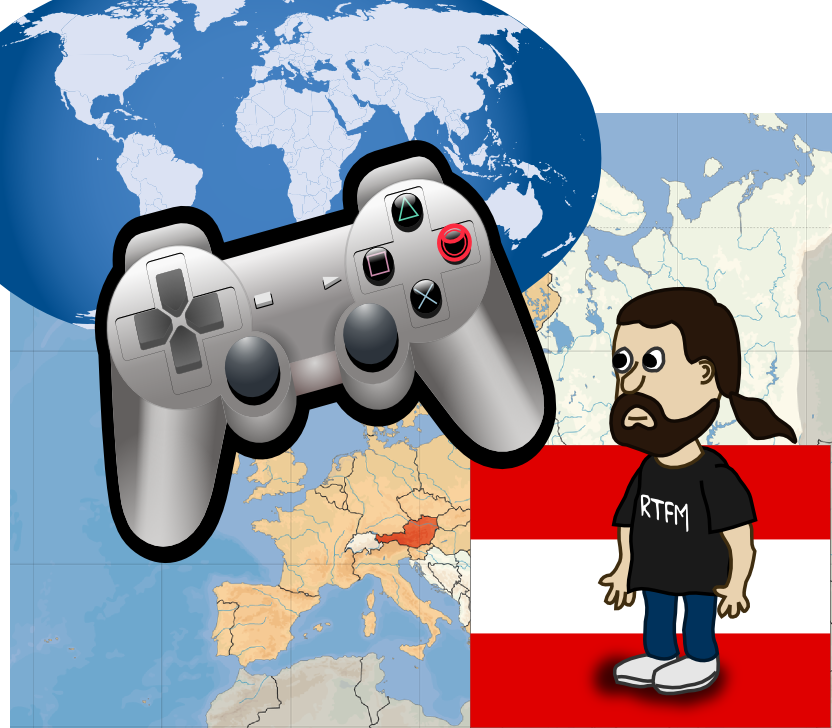
\includegraphics[width=\linewidth]{austrianguy/austrianguy.png} \\
\footnotesize{Bildrechte: \href{https://creativecommons.org/licenses/by-sa/4.0/deed.en}{cc-by-sa} by \href{https://commons.wikimedia.org/wiki/User:David_Liuzzo}{David Liuzzo[3],}\href{https://commons.wikimedia.org/wiki/File:EU_location_AUT.png}{[4],} public domain: \href{http://openclipart.org/detail/175351/playstation-controller-by-matthewhenninger-175351}{[5],}\href{http://openclipart.org/detail/21847/comic-characters:-bearded-guy-by-nicubunu}{[6],}\href{http://openclipart.org/detail/7885/blue-world-map-by-neocreo}{[7],}\href{http://openclipart.org/detail/12612/flag-of-austria-by-anonymous}{[8]}} \\

\includegraphics[width=0.8\linewidth]{austrianguy/molecularmatters.png} \\
\footnotesize{Firmenlogo von Stefan's Firma}
\end{center}

(Beginn der Übersetzung)

Ich dachte es wäre nett hier auf meinem Blog (\href{http://www.altdevblogaday.com/}{\textit{\#altdevblogaday [4]}}) ein Vorstellungs-Posting zu haben; und was wäre dazu besser geeignet als meine Geschichte: von einem Bub aus Österreich (wir sind das Land ohne Kängurus) der in der (Computer)Spiele-Industrie gelandet ist....

\subsection*{Frühe Sucht}

Es begann vor über zwanzig Jahren, als mir mein Vater eine \href{https://de.wikipedia.org/wiki/Colecovision}{\textbf{ColecoVision Spielkonsole}} 
%\pageref{colecovision}ColecoVision Spielkonsole
zeigte - ich war damals circa fünf Jahre alt. Ich habe jetzt noch schönste Erinnerungen daran, damit \textit{Mouse Trap, Donkey Kong} und \textit{Pitfall} auf unserem alten Fernsehgerät zu spielen. Weil die Spiele damals so teuer waren kauften meine Eltern nur ein- oder zweimal im Jahr neue Spiele. Wir waren stolze Besitzer einer Sammlung von acht (8!) Spielen. Trotzdem, wir Kinder spielten damit so oft wir nur konnten.
\begin{center}
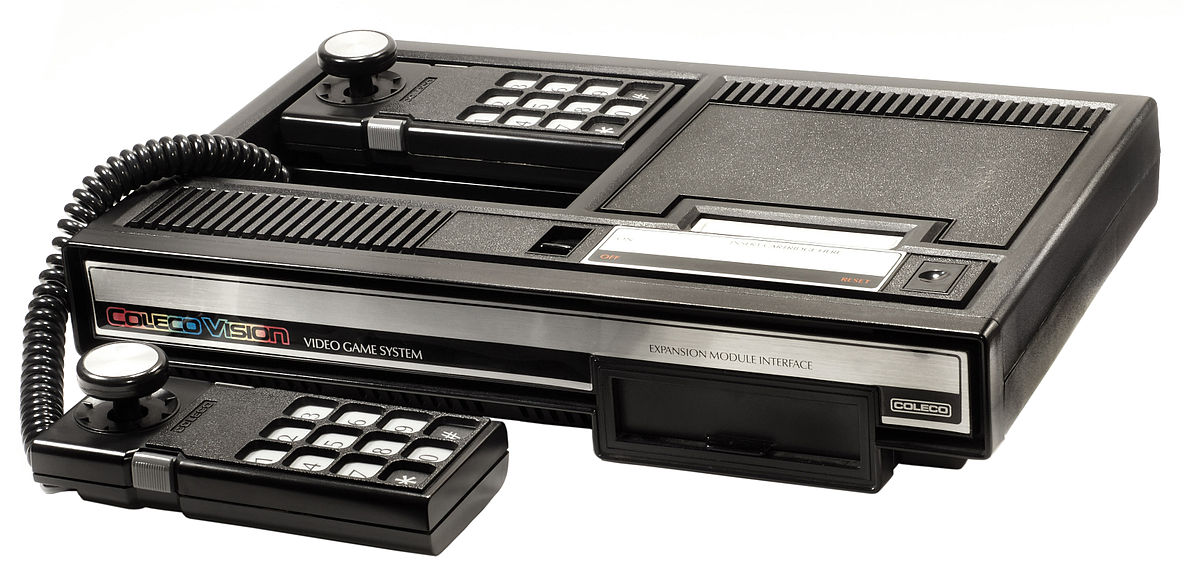
\includegraphics[width=0.9\linewidth]{austrianguy/austrianguy-colecovision.jpg}\\
\footnotesize{ColecoVision-Spielekonsole. Bildrechte: \href{https://commons.wikimedia.org/wiki/File:Coleco-vision-console.jpg}{public domain}}
\end{center}

\subsection*{Commodore 64}

Ein paar Jahre später investierte mein Vater sein Geld in unseren ersten Computer - einen \textbf{Commodore 64}. Ah, der C64 !

Nicht nur gab es für den C64 nicht nur eine riesige Auswahl an Spielen; es war sogar möglich Spiele zu kopieren (Raubkopien waren ein großes Problem). Es gab damals nicht viele offizielle Computerspiele-Verkäufer in Österreich; wir organisierten uns die Spiele durch Kopieren bei Bekannten.  Es stellte sich heraus dass mein Vater einige Leute kannte, und wir spielten unzählig viele verschiedene Spiele. Obwohl das jetzt mehr als zwei Jahrzehnte her ist bekomme ich immer noch eine wohlige Gänsehaut wenn ich an die Spiele denke und speziell an die Melodien vom SID Soundchip des C64...  Jeder von uns nahm Ladezeiten von über zehn Minuten und mehr in Kauf (mit dem Datasette - Kasettenrekorder) einfach weil die Spiele so großartig waren. Der C64 war eine tolle Maschine, ich liebte ihn !

Mit ihm konnte man nicht nur eine ungeheure Menge Computerspiele spielen, es war auch möglich Computerprogramme in der Programmiersprache \textbf{BASIC} zu schreiben und zu starten. Bevor ich überhaupt wusste was Programmieren oder gar BASIC war, zeigte mir mein Vater \textbf{LOGO} (mit \textbf{Turtle Grafik}!), wahrscheinlich mein erster Kontakt mit einer Programmiersprache. Nicht lange danach bekam ich heraus wie man damit einfache Schneeflockenmuster zeichnet mittels den Turtle-Befehlen \textit{turn-left, move-forward, turn-right}. Kurz danach beschäftigte ich mich mit \textbf{BASIC}.

Obwohl ich damals noch nicht in der Lage war höhere Konzepte wie z.B. \textbf{GOSUB} zu verstehen kann ich mich daran erinnern dass es mir Spaß machte einfache \textbf{BASIC} Programme zu schreiben. Immer wenn meine Eltern nicht da waren schlich in ihr Schlafzimmer um den Computer zu benutzen. Immer öfter versuchte ich einfache Konzepte nach zu basteln die ich in anderen Spielen gesehen hatte, um herauszubekommen wie man das macht. Natürlich hatte ich noch keine Ahnung von \textbf{Sprites} oder der C64 Architektur, aber es faszinierte mich den Computer dazu zu bringen etwas zu tun.

\begin{center}
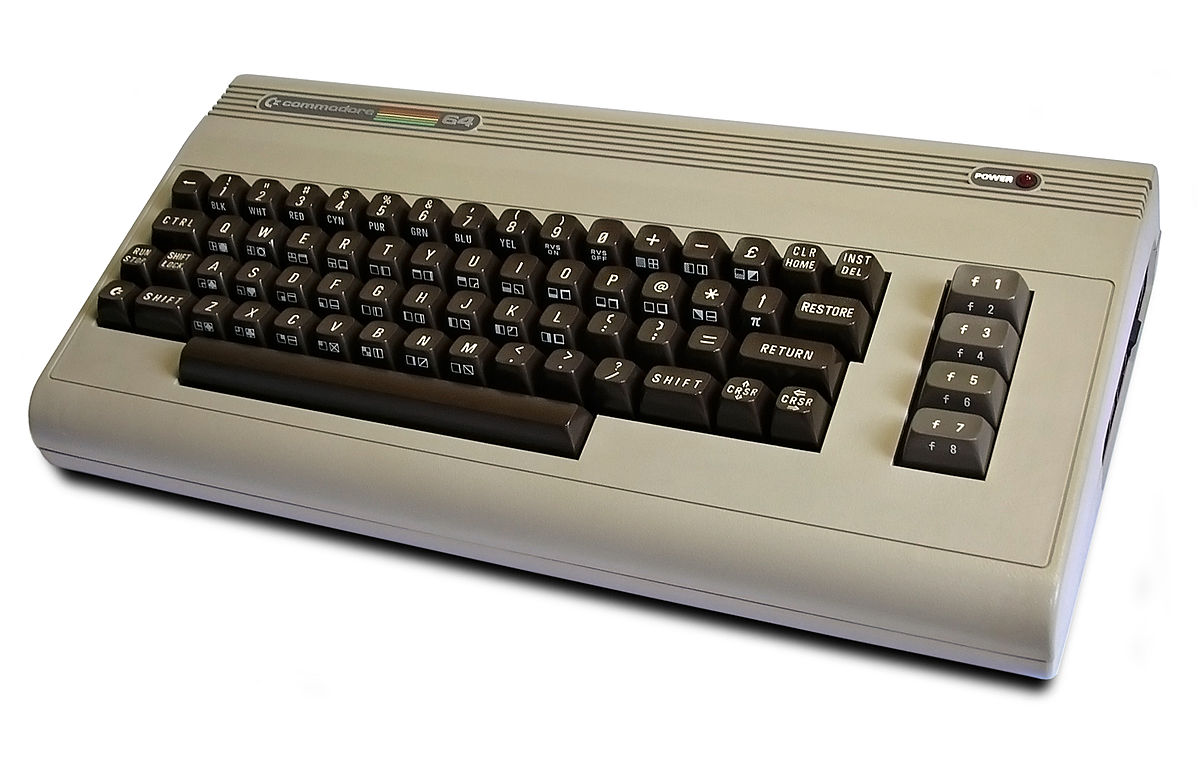
\includegraphics[width=0.9\linewidth]{austrianguy/austrianguy-c64.jpg}\\
\footnotesize{Commodore 64 Heimcomputer. Bildrechte: \href{https://commons.wikimedia.org/wiki/File:Commodore64.jpg}{Bill Betram [5]}, \href{https://creativecommons.org/licenses/by-sa/2.5/deed.en}{cc-by-sa}}
\end{center}

\subsection*{erste Programmier Schritte}

Wenige Jahre später gab mein Vater einen Haufen Geld aus für unseren ersten PC - einen 386er mit 33 MHz. Wir spielten zeitlose Klassiker darauf wie \href{https://de.wikipedia.org/wiki/Wing_Commander_(Computerspiel)}{\textbf{Wing Commander}}, \href{https://de.wikipedia.org/wiki/Syndicate}{\textbf{Syndicate}}, \href{https://de.wikipedia.org/wiki/X-COM}{\textbf{Ufo (X-Com)}}, \href{https://de.wikipedia.org/wiki/Doom}{\textbf{Doom}} - und wir luden Gäste ins Haus ein, um die ganze Nacht Doom Deathmatches zu zocken. Ich kann mich gut daran erinnern wie sehr ich die Leute bewunderte die in der Spiele-Industrie arbeiteten. Ich wusste es ist mein Traum eines Tages ein Spiele-Entwickler zu sein und an solchen Spielen zu arbeiten. Um diese Zeit herum begann mein älterer Bruder mit \textbf{Turbo Pascal} unter \textbf{MS-Dos} zu programmieren. Ich versuchte so viel zu lernen wie ich konnte und nervte ihn andauernd mit Fragen.

\subsection*{PC Demo Szene}

Und dann kam der Tag an dem ich Bekanntschaft mit der \href{https://de.wikipedia.org/wiki/Demoszene}{\textit{PC Demo Szene}} machte.

Dies muss der Punkt gewesen sein in meinem Leben an dem ich anfing mich brennend für Low-Level Programming zu interessieren, für Hardware-Details, für Arbeiten am mit den grundlegendsten Hardwarekomponenten um aus allen Teilen das Letzte herauszuholen. Ich konnte einfach nicht glauben dass so etwas Fantastisches wie Second Reality oder Crystal Dream 2 auf der dem armen 386 meines Vaters möglich war. Diese Demos gehören zu den besten Demos welche jemals gemacht wurden, und ich werde sie nie vergessen. Ich war entflammt. Ich wollte jedes noch so winzige Detail wissen über Texture Mapping, über 3D Algorithmen und mode 13h programming. Aber ich wusste nicht wo ich anfangen sollte. Zum Glück war mein Bruder schon in der Oberstufe und half mir dabei von Vektoren und Matrizen zu lernen sowie generell  programmieren zu lernen.

\begin{center}

\includegraphics[width=0.9\linewidth]{austrianguy/austrianguy-secondreality.jpg}\\
\footnotesize{Second Reality. Bildrechte: \href{https://en.wikipedia.org/wiki/en:public_domain}{public domain}}
\end{center}

\subsection*{Ausbildung}

Ich ging bald selbst in eine HTL und lernte langsam \textbf{C/C++} in meiner Freizeit. Überraschenderweise lernten wir in der Schule fast nie programmieren, nur ein wenig Pascal, was für eine technische Ausbildung eigentlich ungewöhnlich ist. Zu dieser Zeit beschäftigte ich mich immer noch mit Texture-Mapping und Ähnlichem, aber ich kam nie recht voran mit meinem eigenem Spiel. Ich war immer viel zu beeindruckt von den neusten technischen Möglichkeiten und Fachartikeln die ich im Internet las. All das Fachchinesisch über 3D Grafik machte es für mich noch viel mehr interessant. Ich war richtig süchtig nach Technologie und Low-Level Details.

Nach dem HTL Abschluss wusste ich dass ich nicht zurück wollte in einen technischen Beruf, denn dies hatte durch die Schulzeit seinen Reiz für mich verloren. Nicht richtig wissend was und wo ich studieren sollte stolperte ich in ein Computer Science Master Programm an der TU Wien. Ich übersiedelte nach Wien und studierte Computer Graphics und Digital Image Processing.
\begin{center}
    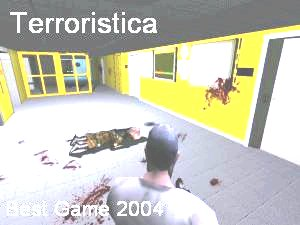
\includegraphics[width=\linewidth]{austrianguy/austrianguy-bestgame2004.jpg}
    \footnotesize{Bildrechte: \href{http://www.cg.tuwien.ac.at/courses/CG23/HallOfFame/2004/}{TU-Wien [6]}}
\end{center}
\subsection*{Erster Lohn}

Zurückblickend weiß ich das manches von dem was mir an der Universität gelehrt wurde nicht ganz meinen Erwartungen entsprach (höflich ausgedrückt) aber manches davon bahnte mir meinen Weg in die Spiele-Industrie. Ich war im 3. Semester von meinem Bachelorprogramm und wir Studenten mussten in Gruppen ein eigenes 3D Spiel mit Open-GL programmieren. Ich wusste dies war meine Chance um meine Fähigkeiten zu erweitern und state-of-the-art 3D Programmierung zu lernen. Und natürlich war ich ganz aus dem Häuschen bei der Idee dass wir unser eigenes Spiel schreiben konnten und dafür noch Noten bekamen, also steckte ich sehr sehr viel Zeit hinein. Unser Spiel gewann den \href{http://www.cg.tuwien.ac.at/courses/CG23/HallOfFame/2004/}{\textit{Best Game of 2004 [6]}} Preis der TU-Wien !

Später im Sommer dieses Jahres kontaktierte ich einen Studienkollegen der in einem österreichischem Entwicklungs-Studio arbeitete (die Szene in Österreich ist winzig klein). Ich fragte ihn ob sein Chef Praktikumsplätze anbietet. Es stellte sich heraus dass mein Kollege nicht mehr für die Firma arbeitete und nichts über deren Praktika wusste. Aber er bot an ein Job-Interview für mich zu arrangieren bei seinem derzeitigem Arbeitgeber, wenn ich interessiert wäre. Und ob ich interessiert war! Ich ergriff die Chance, zeigte mein Portfolio her, zeigte das Spiel welches wir an der Uni gemacht hatten und ich begann am nächsten Montag zu arbeiten.

Nach all den Jahren war ich in der Spiele-Industrie gelandet.

\subsection*{fast forward}

In den letzten 7 Jahren lernte ich extrem viel über Programmieren in meiner Zeit in der Branche. Ich arbeitete mit sehr talentierten, leidenschaftlichen und kreativen Leuten. Und auch wenn ich ein paar Crunch-times erlebte mit über 100 Arbeitsstunden pro Woche, kann ich es von ganzem Herzen empfehlen in der Spiele-Industrie mit Gleichgesinnten zu arbeiten. In die Spiele-Industrie zu gehen war die beste Entscheidung in meinem Leben, es war immer mein Traum.

\subsection*{Fachbegriffe:}
~~~\href{https://de.wikipedia.org/wiki/Colecovision}{\textbf{Colecovsion:}} Eine der ersten Spielekonsolen, produziert von 1982 bis 1984. Sie zeichnete sich dadurch aus dass damals populäre Spielautomaten-Klassiker wie \href{https://de.wikipedia.org/wiki/Donkey_Kong}{Donkey Kong} oder \href{https://de.wikipedia.org/wiki/Zaxxon}{Zaxxon} recht gut auf die Colecovision portiert wurden, da ähnliche Hardware wie in den 'großen' Spieleautomaten verbaut wurde.

\href{https://de.wikipedia.org/wiki/Commodore_64}{\textbf{Commodore 64:}} ein sehr populärer Heimcomputer, mit einer unüberblickbarern Anzahl an (raubkopierten) Spielen. Wurde produziert von 1982 bis 1993. Zum Zeitpunkt seines Erscheinens war er mit 64 Kilobyte (Kb) Ram sehr leistungsstark und hatte für damalige Verhältnisse erstaunliche Grafik- (16 Farben!) und Sound-Fähigkeiten. Mitgeliefert wurde ein BASIC Interpreter von Microsoft.

\href{https://de.wikipedia.org/wiki/BASIC}{\textbf{BASIC}} steht für '\textbf{B}eginner’s \textbf{A}ll-purpose \textbf{S}ymbolic \textbf{I}nstruction Code, eine einfach zu erlernende Programmiersprache war in auf jedem Heimcomputer der 80er Jahre installiert (allerdings in zueinander nicht kompatiblen Dialekten). 

\href{https://de.wikipedia.org/wiki/Logo_(Programmiersprache)}{\textbf{Logo}} eine in den 60er Jahren von \href{https://de.wikipedia.org/wiki/Seymour_Papert}{Seymour Papert}(der unter anderem Tablet-Computer voraussah) entwickelte Programmiersprache, gedacht um \href{http://goo.gl/zJG9WU}{Kindern} Programmieren beizubringen. War ihrere Zeit weit voraus.

\href{https://de.wikipedia.org/wiki/Turtlegraphics}{\textbf{Turtle-Grafik}} simuliert eine Schildkröte, an der ein Stift befestigt ist und die über ein Papier wandert. Man kann der Schildkröte Anweisungen geben (z.B. gehe nach vorn, dreh dich nach links) wodurch Muster auf dem Papier entstehen. Turtle Grafik gibt es heute für verschiedenste Programmiersprachen.

\textbf{GOSUB} 'geh runter' ein Sprungbefehl der Programmiersprache BASIC. Der Computer wurde damit angewiesen ein Unterprogramm auszuführen.

\href{https://de.wikipedia.org/wiki/Sprite_(Computergrafik)}{\textbf{Sprites}}: (engl. Geist) sind bewegliche (2D)-Computergrafiken, z.B. die Spielfiguren beim Spiel 'Pac Man'.  Wenn man eine Briefmarke auf einem Bild herumschiebt entspricht dies der Bewegung eines Sprites in einem Computerspiel.

\href{https://de.wikipedia.org/wiki/Wing_Commander_(Computerspiel)}{\textbf{Wing Commander}} Space-Opera Raumschiffspiel für den, 1990 erschienen.

\href{https://de.wikipedia.org/wiki/Syndicate}{\textbf{Syndicate}} 1993 für MS-Dos-PC'erschienenes taktisches Echtzeit-Computerspiel. Der Spieler steuert in Iso-Grafik eine Gruppe von Agenten seines Konzerns in einem finsteren Cyberpunk Szenario welche Missionen erledigen müssen.

\href{https://de.wikipedia.org/wiki/X-COM}{\textbf{Ufo (X-Com)}} eine Serie von runden-basierten, taktische Computerspielen (ab 1994). Der Spieler steuert eine  kleine Anzahl soldaten um die Erde gegen Außerirdische zu verteidigen und muss sich auch um Forschung, Basenbau und Personalmanagement kümmern. Mehrer Fortsetzungen und Spin-offs, unter anderem das Opens-Source Spiel \url{ufoai.sf.net}

\href{https://de.wikipedia.org/wiki/Doom}{\textbf{Doom}} (1993) einer der ersten netzwerkfähigen 3D Egoshooter von ID Software. Machte den Begriff 'Killerspiel' populär.

\href{https://de.wikipedia.org/wiki/MS_DOS}{\textbf{MS-Dos}} Kommandozeilen-Betriebssystem (ab 1982) von Microsoft für 386er Computer. 

\href{https://de.wikipedia.org/wiki/Turbo_Pascal}{\textbf{Turbo Pascal}} war eine Variante der Programmiersprache Pascal komplett mit Entwicklungsumgebung (Compiler, Editor) und kam von 1983 bis 1993 in immer neuen Versionen heraus. Da deutlich schneller und leistungsfähiger als \textbf{Basic} war Turbo Pascal u.a. vorzüglich geeignet um Programme für das Betriebssystem \textit{MS-Dos} zu schreiben und wurde oft in Schulen als Programmiersprache für den EDV-Unterricht gelehrt. Mit dem Aufkommen des Betriebssystem Windows verlor Turbo Pascal an Bedeutung. Open Source Projekte wie \href{https://de.wikipedia.org/wiki/Free_Pascal}{Free Pascal} werden auch heute noch weiterentwickelt und sind mit  Turbo-Pascal kompatibel.

\href{https://de.wikipedia.org/wiki/C_(Programmiersprache)}{\textbf{C,C++}} Moderne Programmiersprachen.

\subsection*{Download, Feedback:}
\footnotesize{
Download: Ordner \texttt{austrianguy} \Mundus\ \href{http://spielend-programmieren.at/risjournal/001}{spielend-programmieren.at/risjournal/001}\\
Startseite:\\
\href{http://spielend-programmieren.at/de:ris:001:start}{spielend-programmieren.at/de:ris:001:start}\\ 
\Letter\: stefan.reinalter@molecular-matters.com\\}
\normalsize 

\subsection*{Lizenz, Quellen}
\begin{wrapfigure}{l}{2.0cm}

\includegraphics[width=2cm]{austrianguy/ccbysa88x31.png}
\end{wrapfigure}
Dieses Material steht unter der Creative-Commons-Lizenz Namensnennung - Weitergabe unter gleichen Bedingungen 4.0 International. Um eine Kopie dieser Lizenz zu sehen, besuchen Sie \url{http://creativecommons.org/licenses/by-sa/4.0/deed.de}.

\textbf{Quellen:} \\
{[}1{]} \href{http://www.molecular-matters.com}{molecular-matters.com} \\
{[}2{]} \href{http://www.altdevblogaday.com/2011/09/27/how-the-austrian-guy-ended-up-working-in-the-games-industry/}{goo.gl/ohJNMH} \\
{[}3{]} \href{http://spielend-programmieren.at}{spielend-programmieren.at} \\
{[}4{]} \href{http://www.altdevblogaday.com/}{altdevblogadey.com} \\
{[}5{]} \href{https://commons.wikimedia.org/wiki/File:Commodore64.jpg}{goo.gl/pyDNWP} \\
{[}6{]} \href{http://www.cg.tuwien.ac.at/courses/CG23/HallOfFame/2004/}{goo.gl/jUmhba} \\



%\item [3] \url{http://commons.wikimedia.org/wiki/User:David_Liuzzo}
%\item [4] \url{http://commons.wikimedia.org/wiki/File:EU_location_AUT.png}
%\item [5] \url{http://goo.gl/XKyY3Y}
%\


%\item [6] \url{https://openclipart.org/detail/21847/comic-characters:-bearded-guy-by-nicubunu}
%\item [7] \url{http://goo.gl/XoZfl9}
%\item [8] \url{https://openclipart.org/detail/12612/flag-of-austria-by-anonymous}





 

\end{multicols}
\SepRule
%-----------------------------------------------------------
\end{document}